\newpage
\section{Struktura aplikacji}\label{struktura}
\vspace{1cm}
    Aplikacja składa się z dwóch głównych części: 
    \begin{itemize}
        \item Aplikacji mobilnej dostępnej na system Android.
        \item Warstwy back-end zapewnianej przez usługi serwisu Firebase. \\
    \end{itemize}

    Aplikacja mobilna stworzona została zgodnie ze wzorem architektury MVVM (ang. Model-View-Viewmodel, Model-Widok-Viewmodel). Oznacza to, że struktura aplikacji
    podzielona jest na trzy główne elementy: 
    \begin{itemize}
        \item Model — reprezentacja obiektów przechowywanych w bazie danych, warstwa danych.
        \item Widok — warstwa graficzna, wizualna, obsługująca interakcję użytkownika. Reprezentacja modelu w poszczególnych elementach interfejsu użytkownika.
        \item Viewmodel — abstrakcyjny obiekt separujący warstwę danych od warstwy widoku. Zawiera w sobie logikę komunikacji aplikacji z bazą danych,
        oddzielając elementy interfejsu od logiki tej komunikacji.
    \end{itemize}
    
    Firebase~\cite{FIREBASE_MAIN} jest platformą zapewniającą twórcom aplikacji mobilnych i sieciowych różnorodność narzędzi ułatwiających rozwój aplikacji. Platforma jest ściśle powiązana z 
    Google Cloud Platform — główną usługą chmur obliczeniowych Google. Warstwa back-end wykorzystuje dwa produkty oferowane przez Firebase: Cloud Firestore — 
    nierelacyjną bazę danych mającą formę drzewa w pliku o formacie JSON oraz Authentication — narzędzie pozwalające na bezpieczne uwierzytelnianie użytkowników 
    w serwisie zbudowanym na podstawie Firebase. \\ 

    \begin{figure}[!ht]%
        \centering
        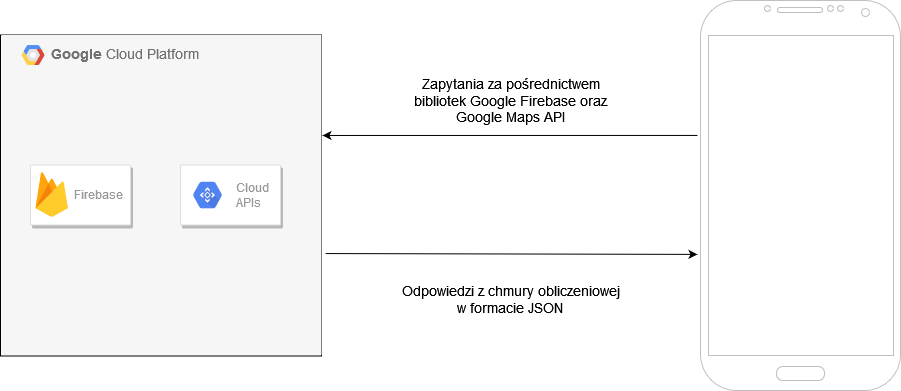
\includegraphics[scale=0.45]{src/comunication with google cloud.png}
        \caption{Komunikacja aplikacji z Chmurą Obliczeniową Google.\label{communication}}
        \qquad
    \end{figure} 

    \subsection{Chmura obliczeniowa Google}\label{google_cloud}
    \vspace{1cm}
    Usługi Chmury Obliczeniowej Google oferowane są za pośrednictwem serwisu Google Cloud Platform. Google Cloud Platform~\cite{GCP_OVERVIEW} jest kompletem narzędzi i usług pozwalających 
    deweloperom budować aplikacje korzystające z tej samej infrastruktury, której firma Google używa do budowania swoich produktów konsumenckich, takich jak Google Search, 
    Gmail, czy YouTube. Google Cloud Platform zapewnia użytkownikom szereg usług typu Infrastruktura Jako Usługa (ang. Infrastructure as a Service, IaaS), Platforma Jako 
    Usługa (ang. Platform as a Service, PaaS) itp. Oznacza to, że Google Cloud Platform jako chmura obliczeniowa ofiaruje swoim użytkownikom sprzęt komputerowy zoptymalizowany do konkretnych
    rozwiązań i pokryty warstwą abstrakcji, jaką jest interfejs chmury obliczeniowej~\cite{DEVHOST}.\\

    Wśród licznych produktów dostępnych na Google Cloud Platform~\cite{GCP_PRODUCTS} można znaleźć m.in. App Engine — Platforma Jako Usługa pozwalająca na wdrażanie aplikacji w językach
    takich jak Java, PHP, czy Python, Compute Engine — Infrastruktura Jako Usługa służąca do tworzenia maszyn wirtualnych, a także wiele narzędzi do przechowywania różnego rodzaju danych,
    wspomagających aplikacje wykorzystujące machine learning, usługi bezpieczeństwa czy liczne narzędzia do zarządzania projektem i analityki. Ponadto w ofercie Google Cloud Platform znajduje się
    kategoria usług \textbf{API Platform}. Daje ona dostęp do obszernej biblioteki Interfejsów Programowania Aplikacji. Należą do niej zarówno API tworzone przez Google, takie jak Cloud 
    Translation API, Google Drive API, czy wykorzystane w niniejszej pracy Maps SDK for Android i Directions API, ale także interfejsy tworzone przez firmy postronne.
    Projekt stworzony na platformie Firebase jest równocześnie projektem Google Cloud platform, co pozwala na proste korzystanie z usług zapewnianych przez oba serwisy. \\

    \vspace{1cm}
    \begin{figure}[!ht]%
        \centering
        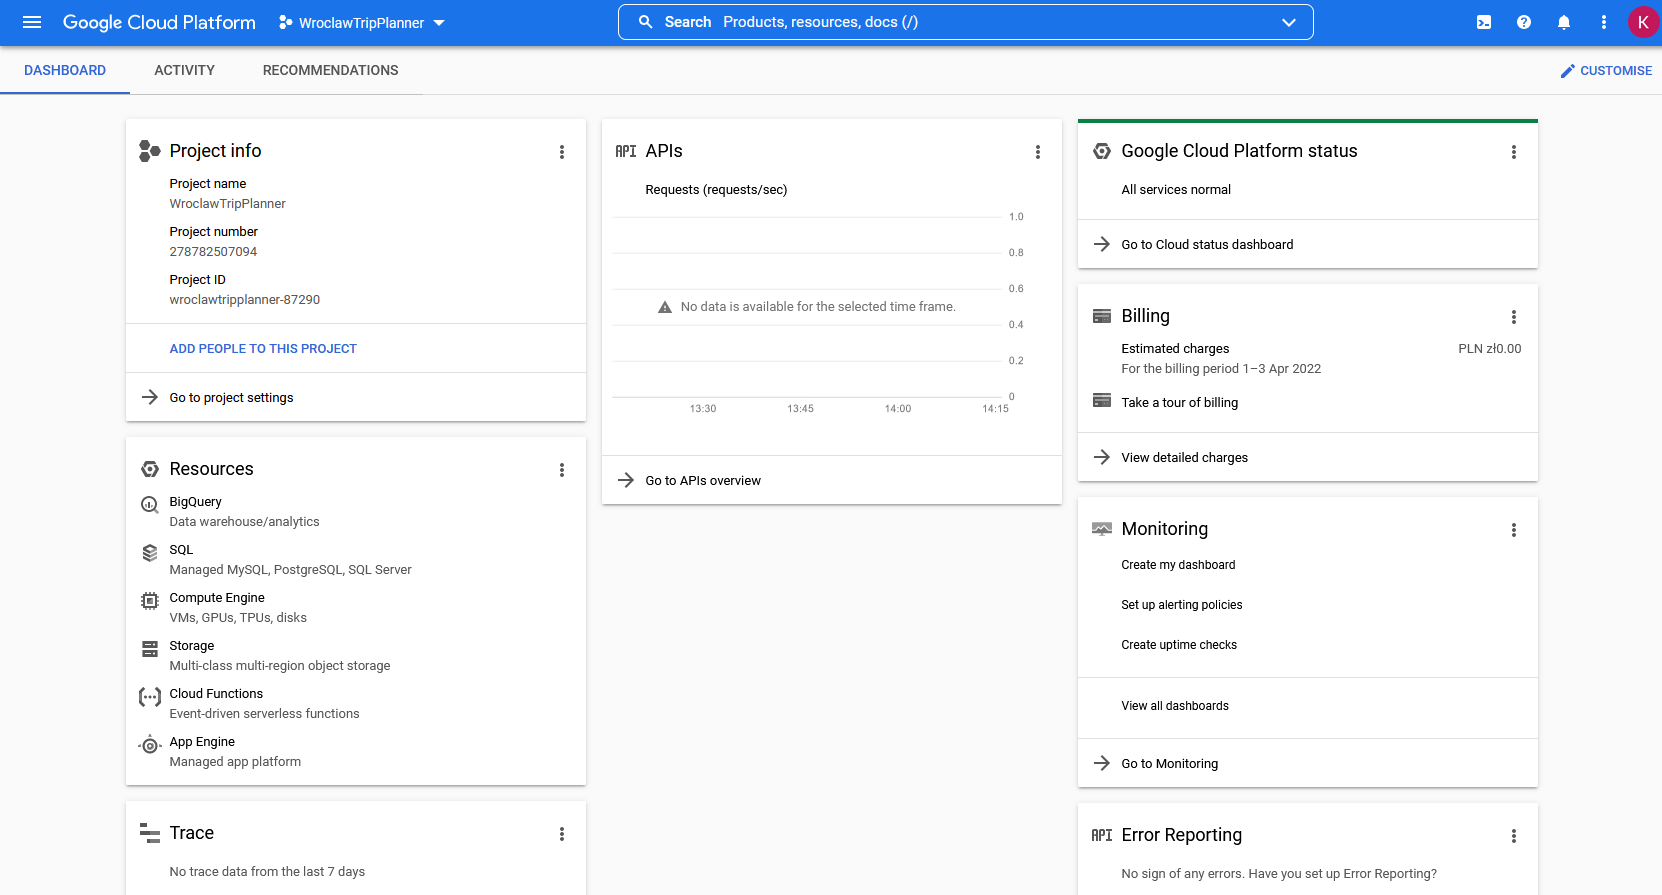
\includegraphics[scale=0.28]{src/gcp console.png}
        \caption{Ekran główny konsoli Google Cloud Platform.\label{gcp_console}}
        \qquad
    \end{figure} 

\newpage
        \subsubsection{Firebase}
        Firebase to rozwijana przez firmę Google platforma dedykowana do tworzenia i rozwijania aplikacji sieciowych i mobilnych. Firebase oferuje swoje narzędzia w formule
        Back-end Jako Usługa. Głównymi usługami Firebase~\cite{FIREBASE_BUILD}, które zostały wykorzystane w omawianej aplikacji to Authentication (pol. Autoryzacja) oraz Realtime 
        Database (pol. Baza danych w czasie rzeczywistym). Poza tymi produktami, których działanie omówione będzie w następnych punktach, Firebase oferuje także takie narzędzia jak 
        Cloud Messaging, pozwalające na proste tworzenie aplikacji do przesyłania komunikatów, Analytics, czyli obszerne narzędzie pozwalające na analizę danych dotyczących zachowania 
        użytkowników, czy Performance, pozwalające na dogłębne monitorowanie wydajności aplikacji. \\ 

        \subsubsection{Firebase Authentication}
        Firebase Authentication~\cite{FIREBASE_AUTH} to jedno z głównych narzędzi Firebase pozwalające twórcy aplikacji na zbudowanie bezpiecznego systemu autoryzacji użytkowników. \\
        Narzędzie to pozwala na zapewnienie użytkownikowi wygodnego systemu logowania, dającego możliwość autoryzacji zarówno za pomocą adresu e-mail, jak i zewnętrznych kont na serwisach takich
        jak Gmail, Twitter, czy Facebook, które mogą posłużyć za wiarygodne źródło autoryzacji. Firebase Authentication pozwala na zaawansowane dostosowanie systemu logowania za pomocą
        e-mail np.\@ poprzez stworzenie autoryzacji kodem wysłanym do użytkownika za pomocą SMS lub e-mail. W niniejszej pracy zastosowana została funkcjonalność logowania poprzez e-mail 
        oraz konto Twitter, jako przykład wykorzystania zewnętrznego konta. Jako że aplikacja nie zapisuje wrażliwych danych użytkownika, takich jak np.\@ historia lokalizacji, nie zostały
        zastosowane żadne dodatkowe formy autoryzacji takie jak link potwierdzający wysłany na adres e-mail użytkownika.
        
        \vspace{1cm}
        \begin{figure}[!ht]%
            \centering
            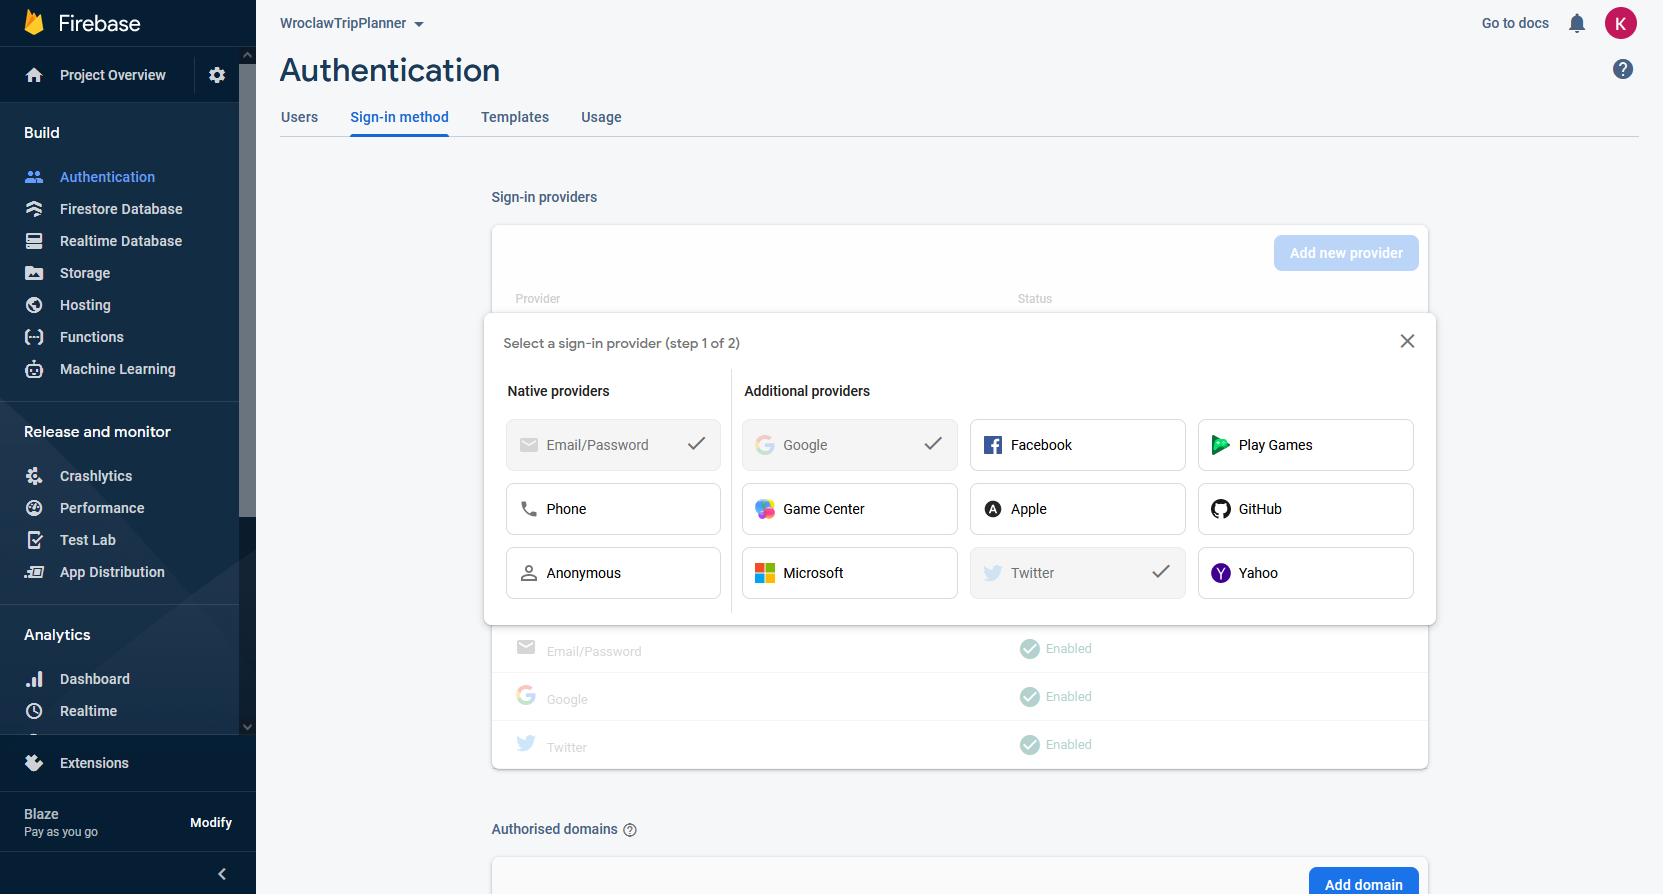
\includegraphics[scale=0.30]{src/firebase auth.png}
            \caption{Ekran wyboru sposobów autoryzacji w konsoli Firebase.\label{firebase_auth}}
            \qquad
        \end{figure} 

\newpage
        \subsubsection{Firebase Cloud Firestore}
        Cloud Firestore~\cite{FIREBASE_FIRESTORE} to produkt Firebase zapewniający twórcy aplikacji skalowalną, nierelacyjną bazę danych pozwalającą na zapisywanie oraz sczytywanie danych w 
        czasie rzeczywistym. Firestore powstał z myślą o zapewnieniu twórcom aplikacji mobilnych i webowych elastycznego narzędzia do tworzenia prostych w rozwoju baz danych. \\
        Do głównych zalet Firestore należą~\cite{FIRESTORE_DOCS}: \\
        
        \noindent Elastyczność — Model danych Firestore zapewnia elastyczną hierarchię i strukturę danych. \\
        
        \noindent Skalowalność — Wykorzystując rozbudowaną infrastrukturę chmury obliczeniowej Google, Firestore jest w stanie dynamicznie zapewniać użytkownikowi m.in.\@ odpowiednie zasoby
        wymagane do bezproblemowego funkcjonowania bazy danych, niezależnie od ilości danych, replikację danych pomiędzy regionami świata, czy gwarancję spójności danych.~\cite{FIRESTORE_SCALE} \\
        
        \noindent Wsparcie off-line — Aplikacje wykorzystujące bazę danych Firestore na bieżąco zapisują stan bazy danych w pamięci podręcznej. Dzięki temu nawet bez dostępu do internetu aplikacja 
        jest w stanie sczytywać i zapisywać informacje, które zostaną zsynchronizowane z chmurą obliczeniową kiedy urządzenie ponownie uzyska dostęp do sieci internetowej. \\
        
        \noindent Aktualizacje w czasie rzeczywistym — odczyt i zapis do bazy danych Firestore następuje w czasie rzeczywistym. Pozwala to aplikacjom wykorzystującym Firestore na nasłuchiwanie zmian 
        w bazie danych i umożliwia natychmiastowe reakcje na zachodzące w niej zmiany. \\

        \noindent Wyraziste zapytania — Firestore pozwala na dokonywanie detalicznych zapytań pozwalających na skomplikowane kombinacje filtrowania i sortowania. Ponadto, baza danych posiada
        system indeksowania zaprojektowany przez Google tak, aby wydajność zapytań była proporcjonalna do rozmiaru wynikowego zestawu, a nie samej bazy danych. \\ 

        Zgodnie z nierelacyjnym modelem danych NoSQL struktury danych są reprezentowane w Cloud Firestore jako Dokumenty~\cite{FIRESTORE_DOCS}. Dokument zawiera w sobie pola mapowane do wartości.
        System ten wspiera liczne typy danych, od prostych łańcuchów znaków i liczb, po bardziej złożone, zagnieżdżone obiekty. Kontenerem zawierającym w sobie dokumenty jest Kolekcja.
        Firestore pozwala także na tworzenie podkolekcji wewnątrz dokumentów. Pozwala to twórcy aplikacji na elastyczne budowanie struktury i hierarchii danych. \\

        Baza danych Firestore umożliwia tworzenie skomplikowanych, ale zarazem wydajnych zapytań dzięki systemowi indeksowania. Indeks bazy danych to struktura danych, 
        często w formie B-drzewa~\cite{DBSYS}, mająca na celu optymalizację prędkości wyszukiwania danych w bazie danych kosztem dodatkowych zapisów danych i miejsca w pamięci, 
        które przechowuję strukturę indeksów. Zamysłem tej struktury jest to, aby uniknąć procesu przeszukiwania każdego wiersza bazy danych w poszukiwaniu wymaganej informacji. Cloud Firestore
        automatycznie generuje indeksy~\cite{FIRESTORE_IDX} zapewniające szybki dostęp do prostych zapytań, np.\' zawierających wyszukiwanie i sortowanie względem jednego pola dokumentu. Dla bardziej 
        skomplikowanych zapytań Firestore oferuje narzędzie dodawania złożonych indeksów. W wypadku kiedy z poziomu aplikacji wyślemy zapytanie wymagające złożonego indeksu, w treści błędu wygenerowany 
        zostanie link automatycznie tworzący pożądany przez twórcę aplikacji indeks. \\

        \vspace{1cm}
        \begin{figure}[!ht]%
            \centering
            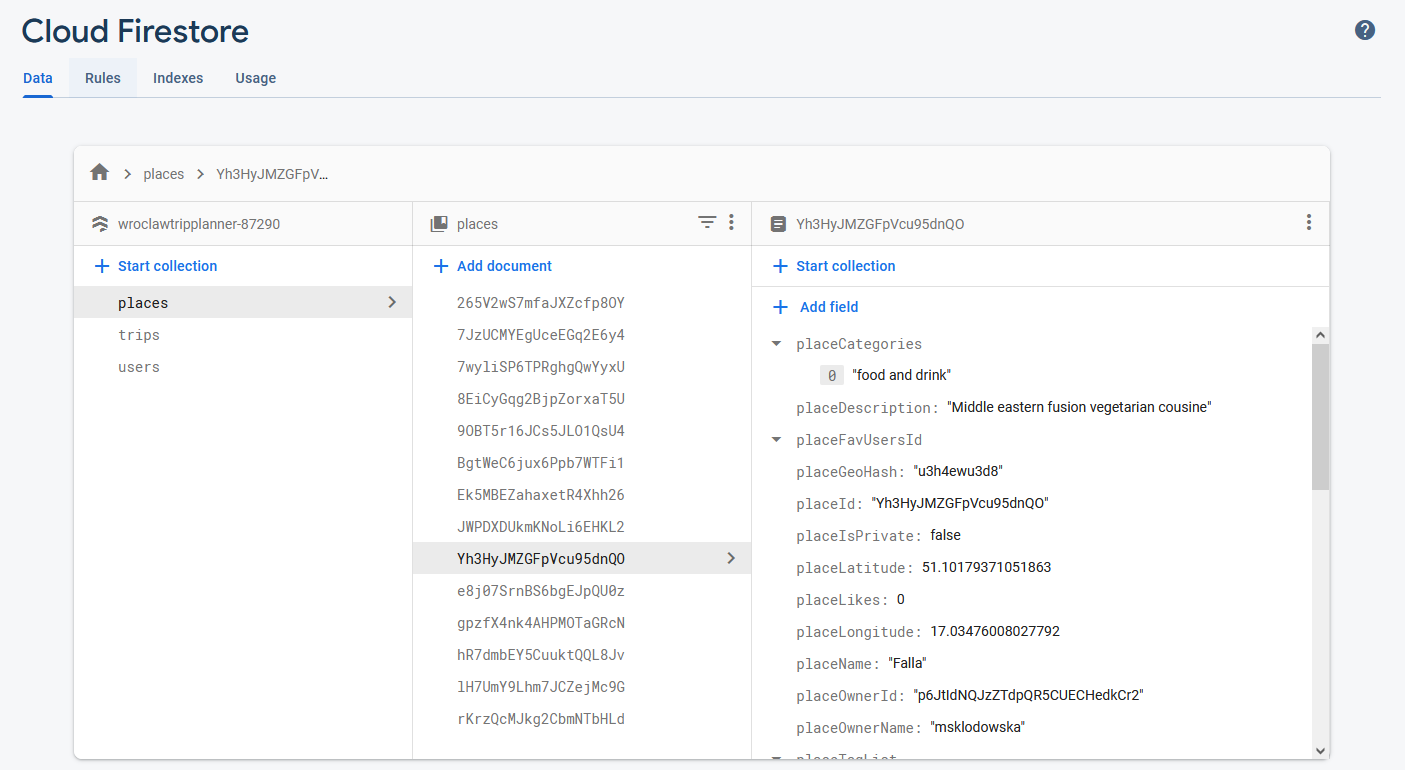
\includegraphics[scale=0.40]{src/firestore_screen.png}
            \caption{Widok bazy danych Cloud Firestore w konsoli Firebase.\label{firestore_screen}}
            \qquad
        \end{figure} 

\newpage
        \subsubsection{Google Maps Platform}
        Google Maps to internetowa aplikacja rozwijana przez Google oferująca szeroki zakres usług nawigacyjnych. Do oferty Google Maps należą m.in.\' zdjęcia satelitarne, mapy ulic, interaktywne,
        panoramiczne zdjęcia ulic w 360°, informacje o stanie ruchu drogowego przekazywane w czasie rzeczywistym i system nawigacyjny powiązany z systemem GPS.\@ Satelitarne zdjęcia Google Maps
        prezentują świat z „widoku ptaka”, a wysokiej rozdzielczości zdjęcia zapewnione są głównie przez fotografię lotniczą. Zdjęcia są aktualizowane przez Google tak często, jak jest to możliwe.
        Google Maps jest także narzędziem, które pozwala na udostępnienie swojego biznesu, np.\' restauracji, czy innego rodzaju firmy. Dodane do bazy danych Google miejsce będzie
        wyświetlać się użytkownikom map, a korzystając z usług reklamowych firmy Google, klient może zapewnić sobie lepsze pozycjonowanie w wyszukiwaniu. Miejsca znajdujące się na mapie Google
        mogą być oceniane i komentowane przez użytkowników. \\

        Google Maps Platform~\cite{MAPS} to rozwijany przez Google zestaw licznych API i Zestawów Narzędzi Programistycznych (ang. Software Development Kit, SDK). Pozwalają one deweloperom na 
        wbudowanie Google Maps w swoją\@ aplikację mobilną bądź internetową oraz na otrzymywanie danych z Google Maps. Google Maps Platform składa się z trzech głównych produktów, w których pogrupowane
        są udostępniane przez firmę API~\cite{MAPS_API}.\\
        Są to: \\
        
        \noindent Maps (Mapy) — Zestaw zawierający w sobie główną funkcjonalność Google Maps Platform — możliwość wyświetlania interaktywnej mapy świata. Do tego zestawu należą: Maps JavaScript API,
        które pozwala na załączenie mapy w aplikacji internetowej, Maps SDK dla systemów Android i iOS, SDK pozwalające na integrację map w aplikacjach mobilnych na obu wymienionych platformach,
        Street View Imagery — API pozwalające na wykorzystanie wykonanych w 360° zdjęć ulic z Google Street View, oraz inne narzędzia związane z widokiem mapy. \\
        
        \noindent Places (Miejsca) — Zestaw wykorzystujący bazę danych miejsc zawartych w Google Maps. Znajdują się w nich takie narzędzia jak Places API pozwalające na pobieranie
        opisów, zdjęć i adresów miejsc w bazie danych Google, Geocoding, pozwalający na dwustronną konwersję pomiędzy koordynatami a adresami lub Autocomplete, przeszukujący bazę miejsc w poszukiwaniu
        takich, które będą pasować do wyszukiwania użytkownika i zostaną zasugerowane w trakcie procesu wyszukiwania. \\

        \noindent Routes (Trasy) — Zestaw narzędzi pomagających wytyczać trasy do pożądanych miejsc. Należą do niego: Directions API, pozwalające na rysowanie na ulicach mapy tras, wskazujących kierunek
        do danych koordynatów, czy Distance Matrix API pozwalające na obliczanie czasu podróży i dystansu pomiędzy wieloma celami podróży.

